\documentclass{article}

\usepackage[letterpaper, portrait, margin=1.5in]{geometry}

\usepackage{fancyhdr}
\usepackage{ragged2e}
\usepackage{graphicx}
\usepackage{caption}
\usepackage{amsmath}
\usepackage{rotating}

\usepackage{listings}
\usepackage{color}

\definecolor{dkgreen}{rgb}{0,0.6,0}
\definecolor{gray}{rgb}{0.5,0.5,0.5}
\definecolor{mauve}{rgb}{0.58,0,0.82}

\lstset{frame=tb,
  language=Java,
  aboveskip=3mm,
  belowskip=3mm,
  showstringspaces=false,
  columns=flexible,
  basicstyle={\small\ttfamily},
  numbers=none,
  numberstyle=\tiny\color{gray},
  keywordstyle=\color{blue},
  commentstyle=\color{dkgreen},
  stringstyle=\color{mauve},
  breaklines=true,
  breakatwhitespace=true,
  tabsize=4
}

\setcounter{secnumdepth}{1}

\usepackage{chngcntr}
\counterwithin{figure}{section}

\renewcommand*{\thepage}{C\arabic{page}}

\pagestyle{fancy}
\lhead{ACME Robotics}
\chead{\#8367}
\rhead{\ifcontents Contents \else Week \thesection \fi}

\newif\ifcontents
\contentstrue

\makeatletter
\renewcommand{\@seccntformat}[1]{}
\makeatother
\begin{document}

\begin{figure}[h!]
\centering
\begin{subfigure}{.45\textwidth}
  \centering
  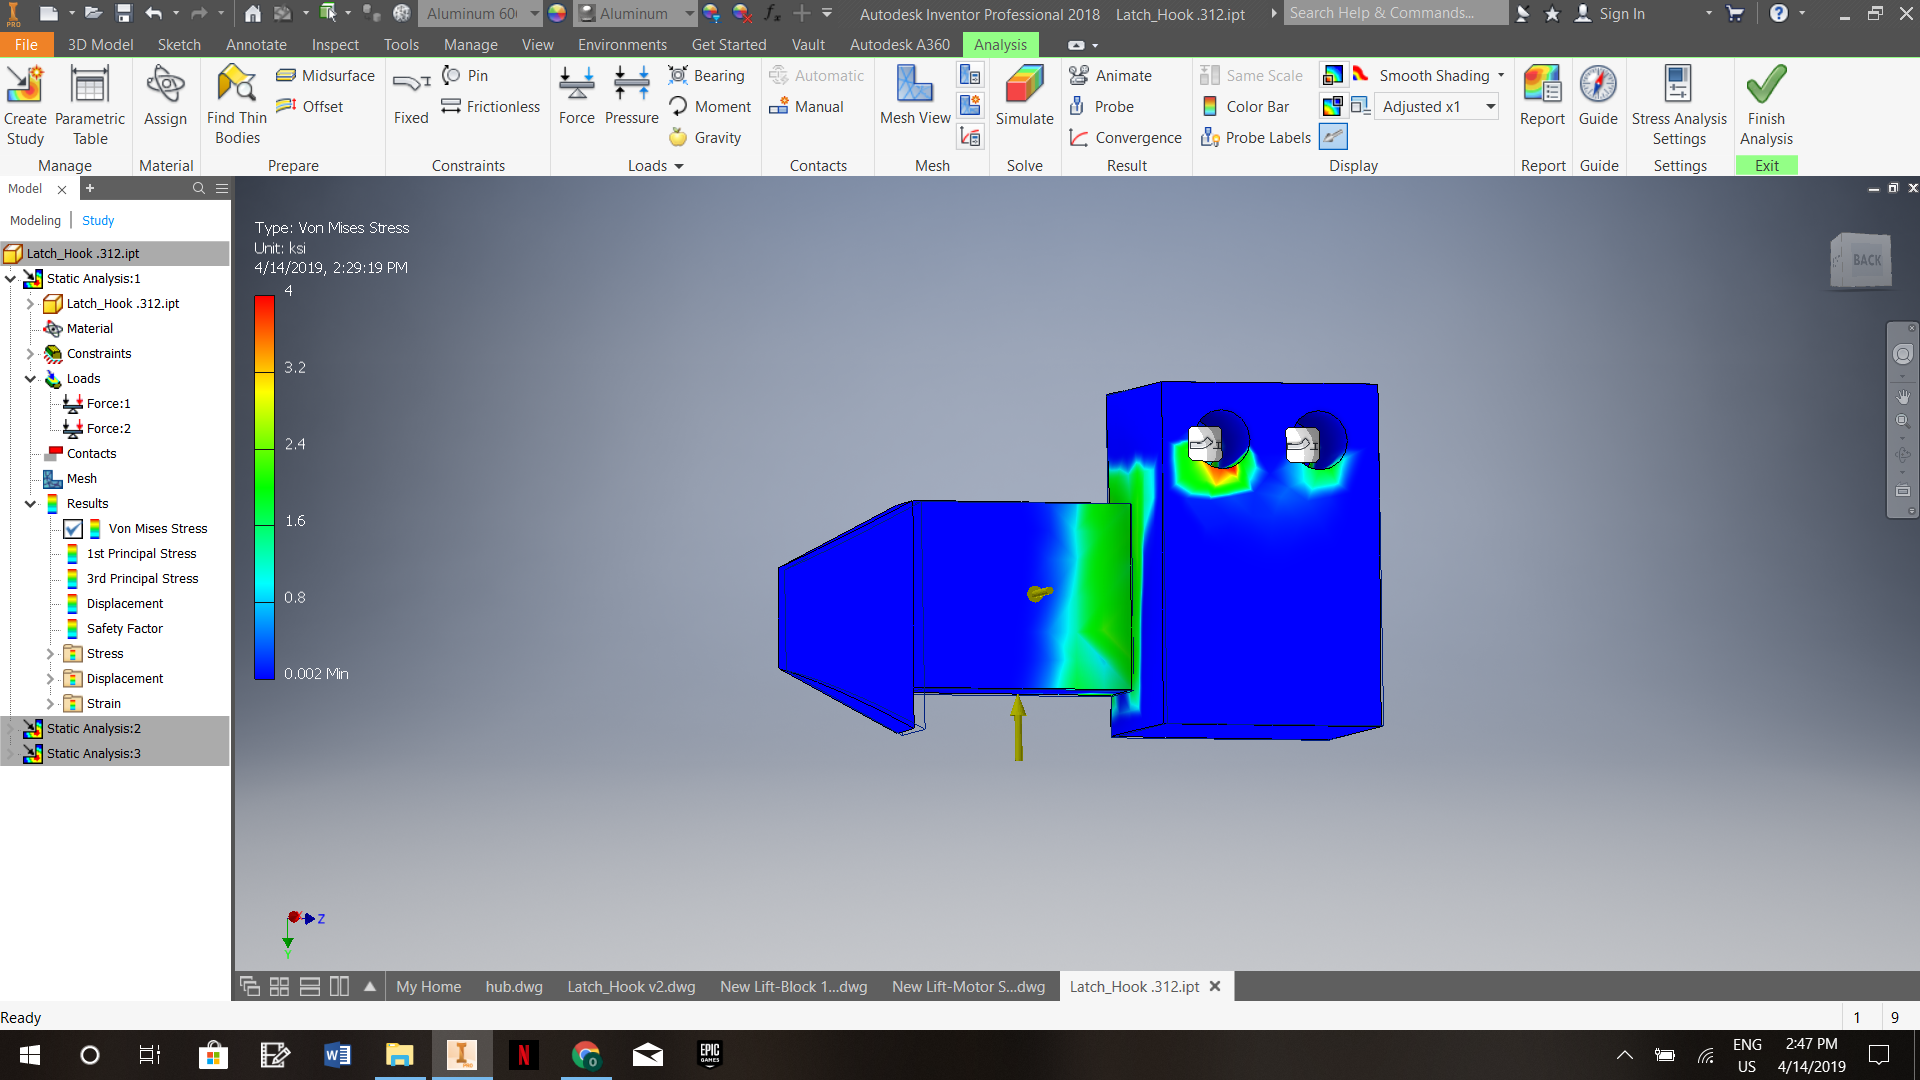
\includegraphics[width=\textwidth]{32_04-08/images/StressLatch.png}
  \caption{Stress Analysis of Machined downed Latch}
  \label{fig:StressLatch}
 \end{subfigure}
\begin{subfigure}{.45\textwidth}
  \centering
  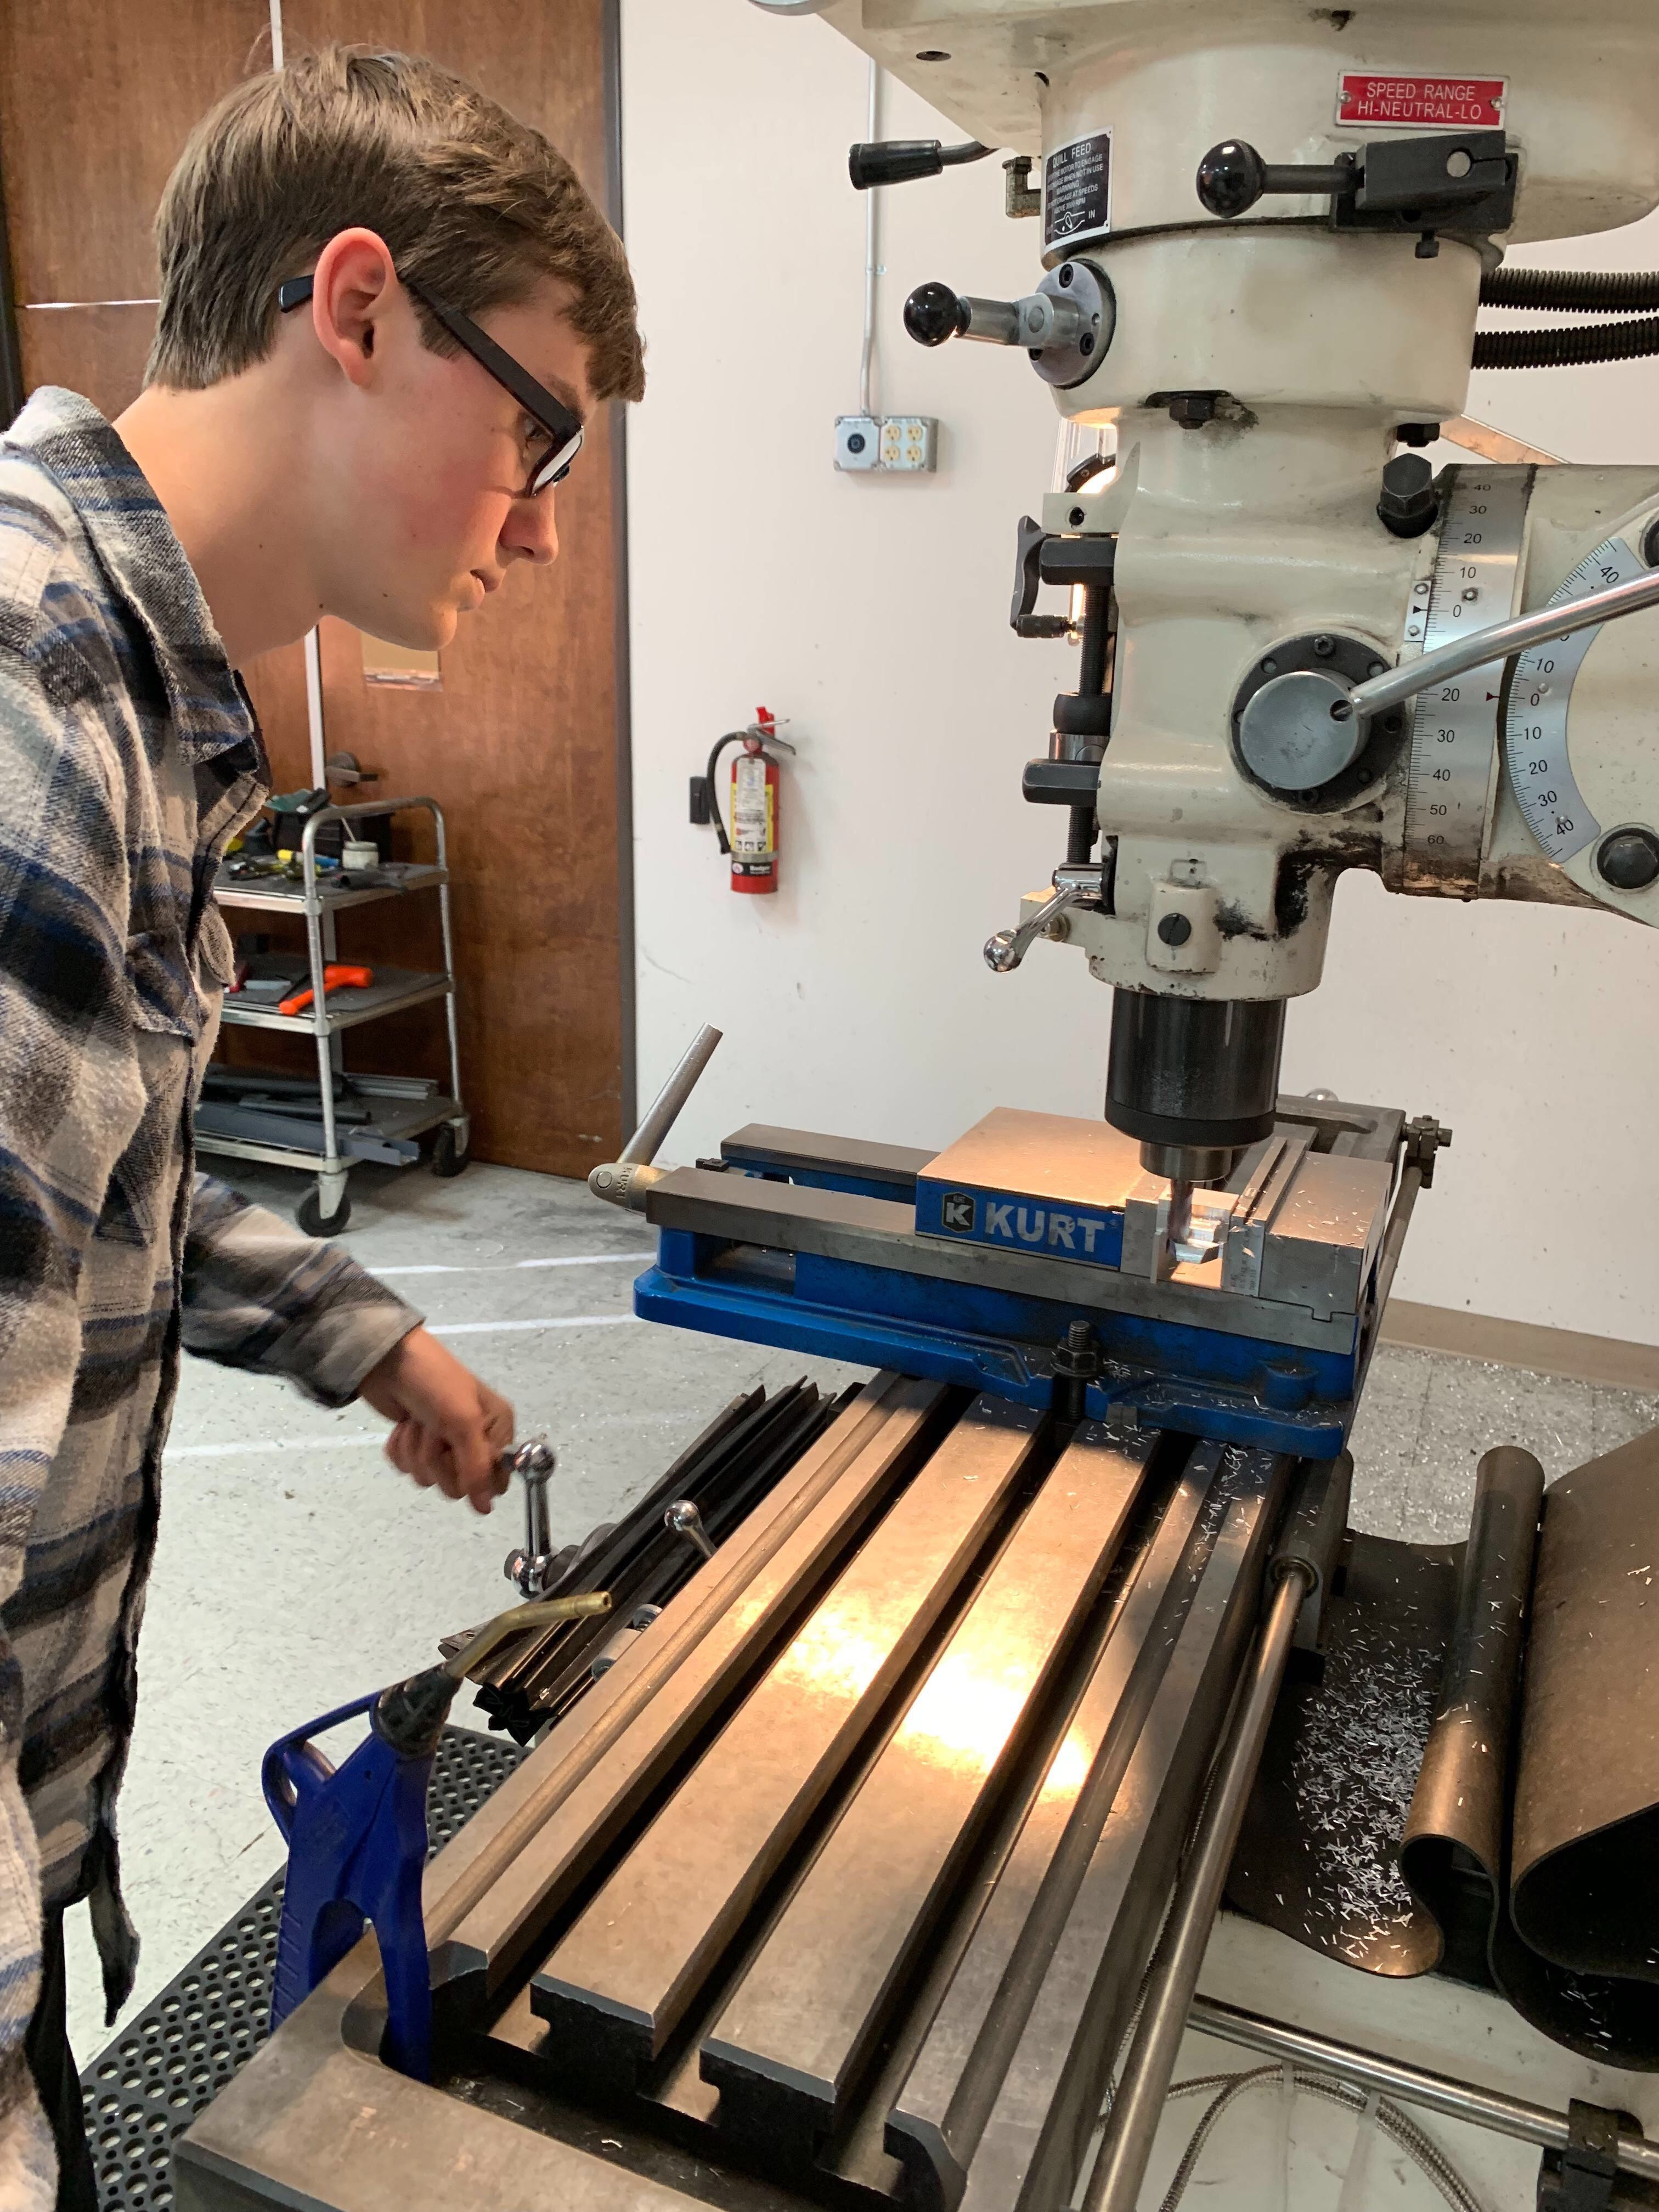
\includegraphics[width=\textwidth]{32_04-08/images/NewLatch.jpg}
  \caption{Ashlin Machining Down Latch}
  \label{fig:MachinLatch}
  \end{subfigure}
  \caption{Latch Analysis and Manufacturing}
  \end{figure}

\subsection{Latch Tuning}
Once the team started drive practice for worlds a problem that Aidan noticed was that latching with the new latch was proving to be difficult. With the new modifications to the latch that raised it higher off the ground, there was less room to latch, making it harder. To fix this, the solution was to mill the inside face down to increase the gap used for latching. Oren ran several stress analyses in Inventor to ensure that the latch could still support the weight of the robot. With data from the stress analysis it was determined that removing 3/16 of an inch would be optimal for ease of use when latching and still strong enough to hold the full weight of the robot. Ashlin then went with Dan to GSS and did the desired modifications. Latching then became significantly easier for the drivers. 

\begin{figure}
    \centering
    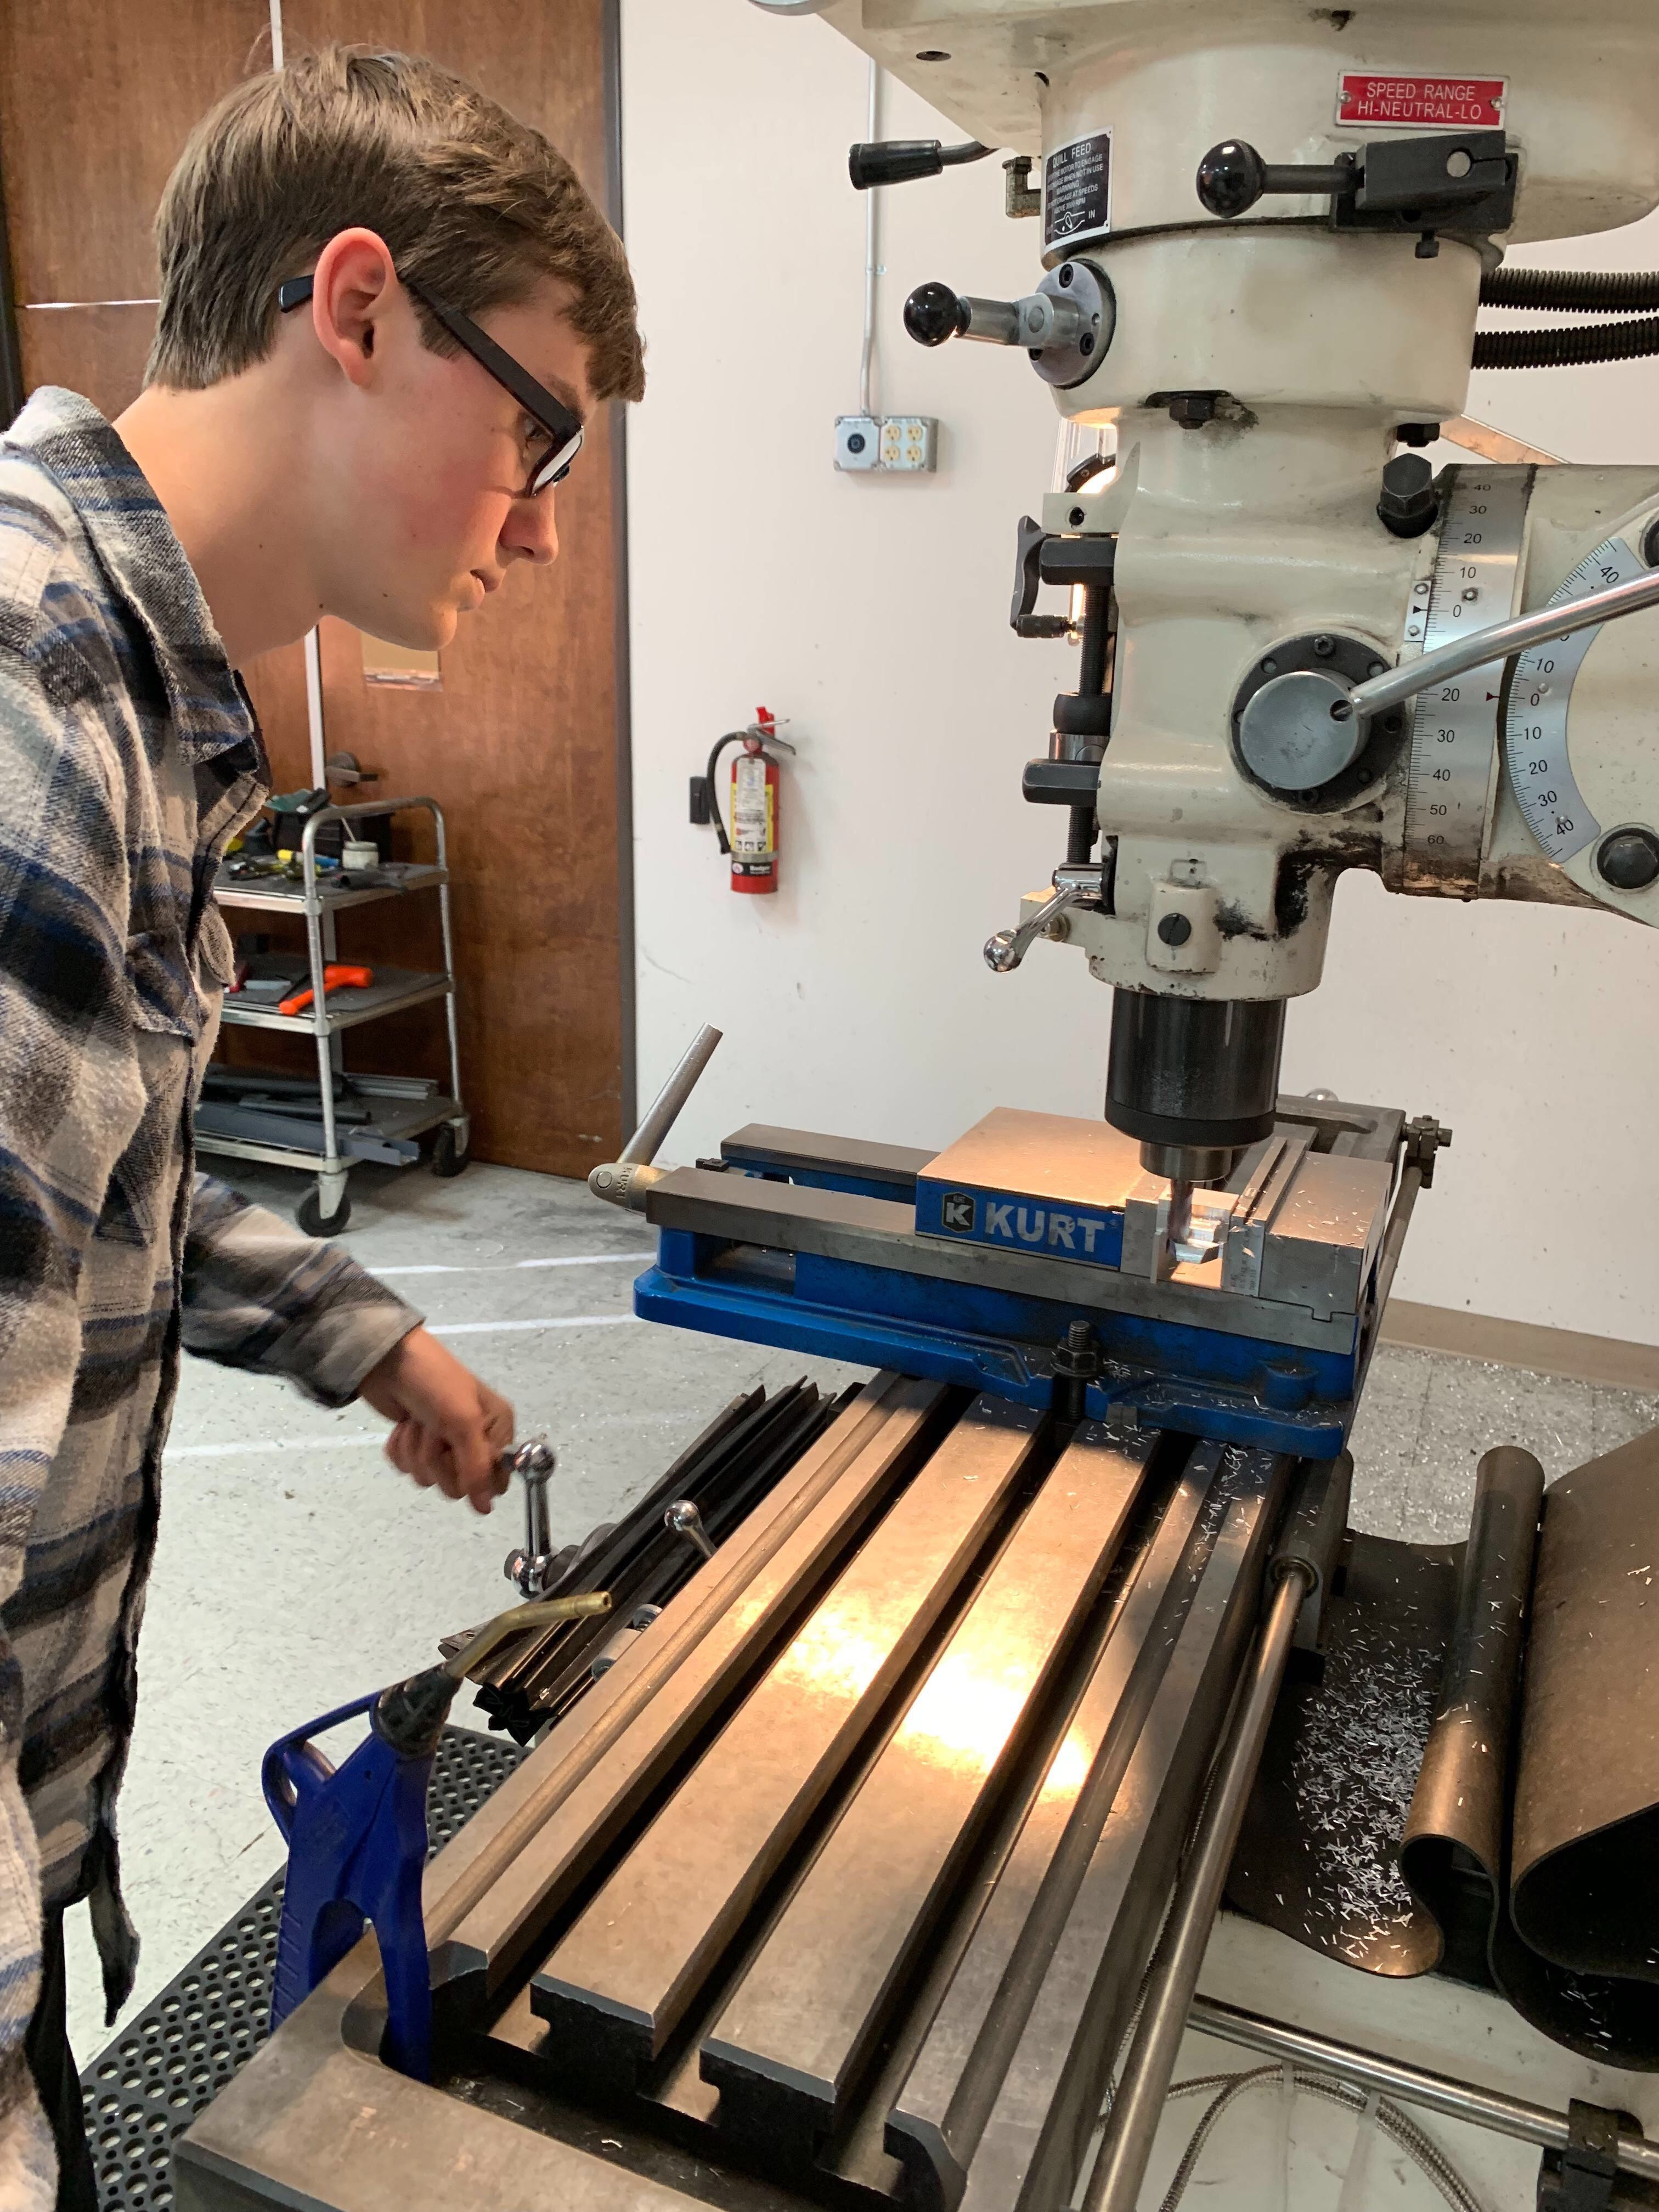
\includegraphics[width= 0.5 \textwidth]{32_04-08/images/ashlinmachining.jpg}
    \caption{Ashlin Modifying the Latch}
    \label{fig:latch}
\end{figure}

\end{document}